\documentclass[conference]{IEEEtran}
\IEEEoverridecommandlockouts
% The preceding line is only needed to identify funding in the first footnote. If that is unneeded, please comment it out.
\usepackage{cite}
\usepackage{amsmath,amssymb,amsfonts}
\usepackage{algorithmic}
\usepackage{graphicx}
\usepackage{textcomp}
\usepackage{xcolor}
\usepackage{array}
\usepackage{url}
\usepackage{multirow}


\def\BibTeX{{\rm B\kern-.05em{\sc i\kern-.025em b}\kern-.08em
    T\kern-.1667em\lower.7ex\hbox{E}\kern-.125emX}}
\begin{document}


\title{Machine Learning Based Detection and Prevention of DDoS Attacks for Cyber Defence }

\author{\IEEEauthorblockN{Arup Kumar Gope }

\IEEEauthorblockA{\textit{Masters of Engineering} \\
\textit{Information Technology}\\
Frankfurt University of Applied Sciences\\
Matriculation No. 1323964\\
arup.gope@stud.fra-uas.de}}
\maketitle
\IEEEpubidadjcol
\sloppy
\begin{abstract}
Machine learning is important in cybersecurity because it allows network administrators to use predictive analytics to secure their websites, servers, and networks.  This research studies the use of machine learning approaches to detect Distributed Denial of Service (DDoS) attacks on lab data.  To test their detective performance, we used three classification algorithms: Random Forest, Logistic Regression, and Neural Network.  The results show that the Random Forest and Neural Network classifiers achieve F1 Scores of 0.9989 and 0.9838, respectively, and Logistic Regression 0.8838.  These studies indicate the successful use of machine learning for early DDoS detection.


\textbf{keywords - }{DDoS, Machine Learning, Random Forest. Logistic Regression, Neural Network.}

\end{abstract}
%
%
%
\section{INTRODUCTION}

This is an era in which a person is growing increasingly vulnerable to a cyber attack.  Various technological precautions have been implemented to prevent cyber attacks or people from becoming victims of malicious attacks.  Recent statistics show that DDoS attacks account for a significant portion of network attacks ~\cite{1}.  Several studies have been undertaken on detection and prevention measures.  Machine learning is an important tool for detecting cyber assaults.  This paper examines Distributed Denial of Service (DDOS) attacks.  The primary premise of a DDoS attack is to overload the target's network infrastructure~\cite{2}.  Although the usage of attacks using DDoS changes there are three major stages: preparation, implementation, and exploitation.  Attackers organize the attack in the first stage, accumulating enough resources to exploit the computers and devices that will be included in the botnet through the development of an effective attack.  A malicious assault that overwhelms the target with unexpected data flow such as phony HTTP requests, UDP packets, and multiple TCP connections.  This enables the attacker to exploit vulnerabilities in the target infrastructure or redirect traffic through a botnet controlled by him.  During the exploitation phase, attackers analyze the attack's effectiveness and customize their tactics as needed.  They may be able bypass detection or mitigation by security measures through modifying tactics~\cite{3}.  

DDoS attacks can cause major service disruptions, limiting the availability and accessibility of targeted services.  The operational disruptions created by these attacks can have a negative effect on business revenue, company reputation, and user trust.  Furthermore, DDoS attacks are frequently employed as a form of extortion against the target firm or organization, with attackers demanding payment to halt the attack.  Furthermore, denial of service attacks can be used by attackers to divert attention towards other security breaches, allowing them to commit crimes like data theft or system disruption.  DDoS attacks thus cause not just financial and operational losses, but also a threat to the target organization's information security and reputation~\cite{4}.  As a result, we must develop techniques to prevent this from happening. A possible approach for preventing DDoS attacks is to use machine learning.
\begin{figure}[ht]
    \centering
    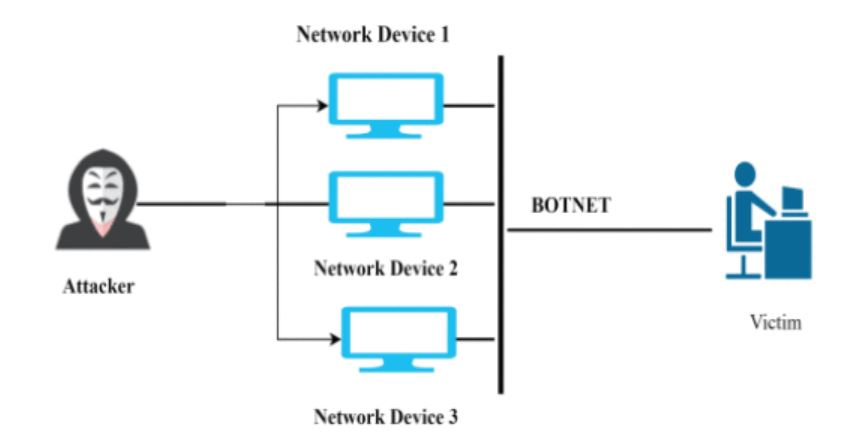
\includegraphics[height=5cm,width=8.5cm]{DDoS_Photo.JPG}
    \caption{DDoS Attack~\cite{11}} 
    \label{fig1}
\end{figure}

Machine learning is a branch of artificial intelligence that focuses on creating computer systems that are capable of learning from data, spot patterns, and make decisions with little or no human intervention.  In simple terms, machine learning attempt to allow computers to perform activities that do not require detailed programming~\cite{5}.  Machine learning involves many different kinds of concepts and methodologies.  One of these is algorithmic.  A machine learning algorithm is a collection of calculations and statistics used by computers to identify patterns in data, make decisions, or anticipate how they will do so.  The primary goal of machine learning algorithms is to develop models that can be used to generalize known training patterns to new data that have never been encountered before~\cite{6}.  Choosing an algorithm appropriate for the type of data and the situation at hand is critical.  Because the appropriate algorithm can considerably improve the model's performance.  As a result, in this research, we will analyze three algorithms based on their accuracy, precision, recall, and F1 score.

\section{Background on DDoS Attacks and Mitigation Strategies}

In the field of cybersecurity, Distributed Denial-of-Service (DDoS) attacks are among the most disruptive and forceful threats available. These attacks are meant to overwhelm the resources of targeted systems, networks, or services, thereby denying access to authorized users. Examining their structure, classifications, and current defense mechanisms will help one to grasp their influence and create reasonable countermeasures.~\cite{12}

\subsection*{1) Nature of DDoS Attacks}
Usually starting from several hacked machines, known as a botnet, DDoS attacks let attackers create massive quantities of traffic together from distributed sources. Unlike conventional Denial-of-Service (DoS) attacks starting from a single source, this distributed character makes identification, filtering, and minimizing far more challenging.

\begin{figure}[htbp]
\centerline{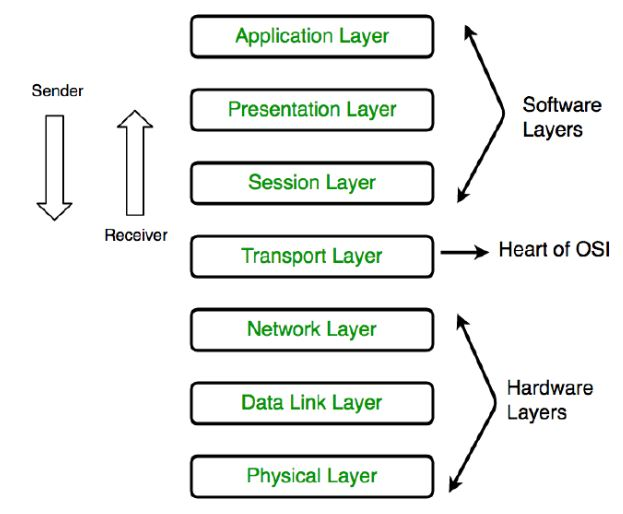
\includegraphics[height=5cm,width=7cm]{OSIModel.JPG}}
\caption{OSI Model Layers ~\cite{13}}
\label{fig:OSI}
\end{figure}

\subsection*{2) Classification of DDoS Attacks}
In general, DDoS attacks are categorized according to the OSI model layer they target. Different network or system resources are used by each class, which requires different mitigation techniques. Volume-based attacks, protocol-based attacks, and application-layer attacks are some of these types. ~\cite{12}

\begin{itemize}
    \item \textbf{Volume-Based Attacks:} By generating huge amounts of traffic, these attacks target to use up all of the targeted system's or service's bandwidth. UDP floods, ICMP floods, and amplification attacks (such as DNS and NTP amplification) are typical examples. The goal of these attacks is to use up the entire bandwidth accessible by sending massive payloads or continuous data packets. Bits per second (bps) are used for measuring such attacks.

    \begin{figure}[htbp]
    \centerline{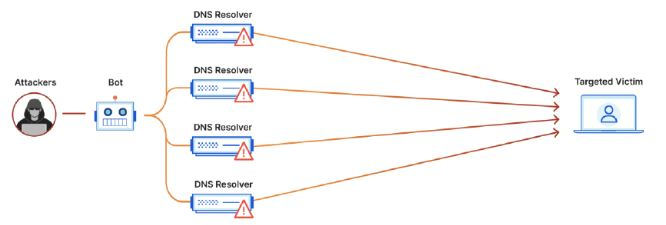
\includegraphics[height=4cm,width=7cm]{VolumeBasedAttack.JPG}}
    \caption{Volume-Based Attack~\cite{13}}
    \label{fig:volume_attack}
    \end{figure}

    \item \textbf{Protocol Attacks:} These target flaws in Layer 3 and Layer 4 protocols to take advantage of server resources or intermediary communication devices like firewalls and load balancers. SYN floods, Smurf attacks, and Ping of Death are examples of common types. The aim of these attacks is to destroy resources like networking hardware or server connection tables. Usually, they are measured in packets per second (pps).

    \begin{figure}[htbp]
    \centerline{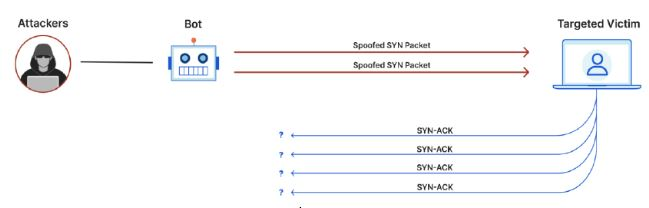
\includegraphics[height=4cm,width=7cm]{ProtocolAttack.JPG}}
    \caption{Protocol-Based Attack~\cite{13}}
    \label{fig:protocol_attack}
    \end{figure}

    \item \textbf{Application-Layer Attacks:} These are the most advanced kinds of DDoS attacks since they replicate valid requests to target particular applications or services. These include DNS query floods, Slowloris, and HTTP floods. By flooding web servers, application servers, or databases with what looks to be real traffic, application-layer attacks seek to bring them down. They are more difficult to identify using traditional firewalls and are measured in requests per second (rps).

    \begin{figure}[htbp]
    \centerline{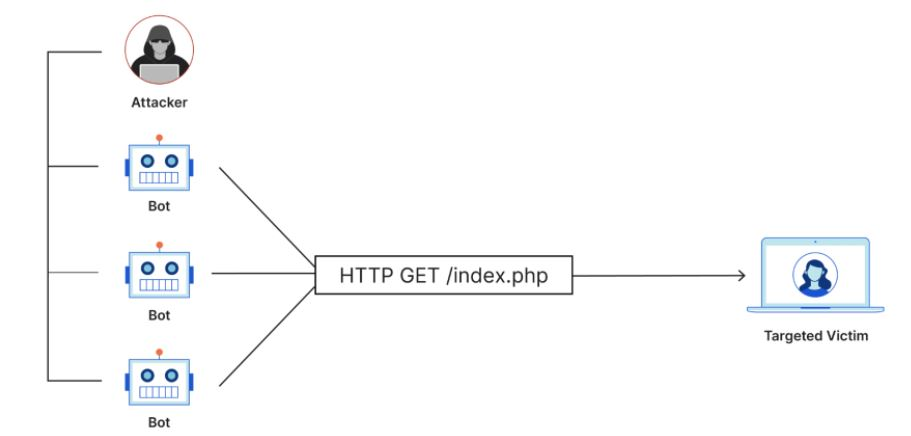
\includegraphics[height=4cm,width=7cm]{ApplicationAttack.JPG}}
    \caption{Application-Based Attack~\cite{13}}
    \label{fig:application_attack}
    \end{figure}
\end{itemize}



\subsection*{3) Mitigation Techniques}

Effective DDoS attack mitigation calls for a multi-layered, flexible strategy that takes into consideration the unique characteristics of the attack. Volume-based, protocol-based, and application-layer attacks are the three main categories of DDoS attacks that are targeted by the strategies listed below ~\cite{14}.

\begin{itemize}
    \item \textbf{For Volume-Based Attacks:}  
    These attacks aim to saturate the bandwidth of a target by generating extremely large volumes of traffic. To mitigate such attacks, several strategies can be employed:
    \begin{itemize}
        \item \textit{Rate Limiting:} Controls down the traffic flood by limiting the number of requests a server accepts in a specified amount of time.
        \item \textit{Bandwidth Over-Provisioning:} Involves setting aside more bandwidth than is normally required in order to handle unforeseen spikes in traffic.
        \item \textit{Traffic Filtering and Scrubbing:} Reroutes traffic via scrubbing centers, which distinguish between malicious and authentic packets.
        \item \textit{Anomaly Detection Systems:} To identify abrupt changes in volume and initiate an automated defense or alert, use traffic baselining and behavioral analytics.
    \end{itemize}

    \item \textbf{For Protocol Attacks:}  
    These take advantage of server resources like connection tables or packet processing power and target flaws in protocols like TCP/IP. Among the defensive strategies are:
    \begin{itemize}
        \item \textit{Stateful Firewalls and Intrusion Prevention Systems (IPS):} Monitor to identify and stop unauthorized connection requests, particularly SYN floods.
        \item \textit{SYN Cookies:} Used to validate TCP handshake attempts before allocating server resources.
        \item \textit{Deep Packet Inspection (DPI):} Finds spoofed or malformed packets by examining the headers and content of the packet.
        \item \textit{Protocol Rate-Limiting:} Restricts particular traffic types that are known to be used in DDoS protocol attacks.
    \end{itemize}

    \item \textbf{For Application-Layer Attacks:}  
    Because they follow real user behavior and target high-level services like HTTP, DNS, or SMTP, these attacks are the hardest to identify. Defense tactics consist of:

    \begin{itemize}
        \item \textit{Web Application Firewalls (WAFs):} Inspect HTTP requests to detect and block malicious payloads or abnormal patterns. ~\cite{15}
        \item \textit{Content Delivery Networks (CDNs):} Content Delivery Networks To absorb and divert attack traffic before it reaches the origin server, geographically distribute application resources.
        \item \textit{Bot Management Systems:} To differentiate between bots and real users, use machine learning and challenge-response tests (such as CAPTCHA) ~\cite{16}.
        \item \textit{Rate Limiting and IP Reputation Filtering:} Blocks traffic from known malicious IP addresses or geolocations and lowers request rates per user.
    \end{itemize}

    \item \textbf{General Strategies:}  
    Beyond attack-specific defenses, a number of general practices contribute to overall DDoS resilience:
    \begin{itemize}
        \item \textit{Blackholing and Sinkholing:} Sinkholing reroutes malicious traffic to a non-operational IP for analysis, whereas blackholing completely drops it.
        \item \textit{Geographic and ASN Filtering:} Blocks or filters requests coming from networks or areas known to be the source of attacks.
        \item \textit{Cloud-Based DDoS Protection Services:} Platforms like Cloudflare, AWS Shield, and Akamai offer reactive and scalable defenses that use globally dispersed infrastructure to withstand massive attacks.
        \item \textit{Redundancy and Load Balancing:}Distributes workloads and traffic among several servers or locations, increasing system resilience.
    \end{itemize}
\end{itemize}



\subsection*{4) Challenges and the Role of Machine Learning}
DDoS attacks keep increasing in scope and complexity even with continuous efforts. Attackers often modify their methods to evade conventional security systems, hence stressing the need for more clever and flexible defense systems. In response, proactive DDoS detection has become significantly assisted by machine learning. ML-based systems can learn traffic behavior patterns, differentiate between normal and abnormal flows, and change with time to fit evolving threats. The application of machine learning classifiers to enhance DDoS traffic detection and classification in modern network systems will be examined in this work.



\section{MACHINE LEARNING MODELS}

Machine learning (ML) is an area of artificial intelligence that allows computers to understand patterns and make data-driven decisions without explicitly programming each task.  Instead of manually coding each rule or instruction, ML systems enhance performance by learning from previous examples.  This method is especially useful for complex projects when manually recording all conceivable outcomes is impossible.

Machine learning involves developing and implementing algorithms that can generalize from previous data.  Simple tasks can be directly coded, but more complicated challenges require systems that can learn and adapt over time. By exposing the computer to labeled or unlabeled datasets, it can infer rules or patterns that can then be applied to new data.~\cite{7}

\subsection{Random Forest}
Random Forest is an ensemble-based supervised learning algorithm that generates a large number of decision trees during training and returns the majority vote (mode) for classification tasks.  It improves forecast accuracy and reduces overfitting by combining the outputs of numerous trees, each based on a different random subset of the data and characteristics.  In this study, we used the Scikit-learn library's \texttt{RandomForestClassifier} module to create a Random Forest classifier.  A total of 100 decision trees were built (\texttt{n\_estimators=100}), with a maximum depth of 15 (\texttt{max\_depth=15}) to balance model complexity with generalization.  By limiting tree depth, we expected to avoid the overfitting while maintaining optimal performance.  To improve computational efficiency, the model was trained on all CPU cores (\texttt{n\_jobs=-1}), using a fixed random seed (\texttt{random\_state=42}) to ensure accuracy.  This method is especially robust in high-dimensional data spaces, making it ideal for dealing with non-linear connections and feature interactions prevalent in network traffic data. This approach is particularly robust in high-dimensional data spaces and is well-suited for handling non-linear relationships and feature interactions commonly found in network traffic data.

\subsection{Logistic Regression}
Binary classification problems can benefit from the well-known statistical method logistic regression. Using a logistic (sigmoid) function, it models the likelihood of a categorical dependent variable depending on one or more independent variables. In the framework of this work, a baseline classifier—logistic regression—was used to offer a benchmark for more advanced machine learning models. The Logistic Regression class from Scikit-learn was used in implementation. The number of iterations was increased to 1000 (\texttt{max\_iter=1000}) to guarantee that the optimization algorithm effectively converged. Logistic regression's simplicity, low computational cost, and interpretability make it perfect for first investigation. Despite its linear decision boundary, it can still perform competitively when feature engineering and data scaling are properly applied, as was done using the \texttt{RobustScaler} in preprocessing.

\subsection{Neural Network (Multi-Layer Perceptron)}
A Multi-Layer Perceptron (MLP) classifier was used in a neural network model to capture increasingly complicated, non-linear relationships in the data. Two hidden layers totaling 100 and 50 neurons respectively made up the architecture (\texttt{hidden\_layer\_sizes=(100, 50)}). This framework lets the model learn hierarchical versions of the input data. With \texttt{early\_stopping=True} turned on to track validation performance and stop training when no more improvement was seen, training ran for a maximum of 500 iterations (\texttt{max\_iter=500}). Particularly in a somewhat small dataset, this helps reduce overfitting. The neural network was built with an adaptive learning rate and backpropagation supported \texttt{MLPClassifier} from Scikit-learn. The MLP model was selected because it could replicate complex patterns in network traffic, so perhaps allowing more precise identification of small DDoS attack signatures.



\section{Work Flow}

The workflow of this project follows a step-by-step process for detecting Distributed Denial-of-Service (DDoS) attacks using machine learning. It begins with gathering network traffic data from a publicly accessible dataset comprising both attack-related and normal activity. Following collecting data, any missing or incorrect data are removed to ensure accurate and suitable information. Then the labels in the dataset—which indicate whether the traffic is normal or an attack—are divided into two categories: one for regular traffic and another for DDoS attacks. Once cleaned, the data is ready for analysis by means of consistent formatting and value scaling, so treating all features fairly throughout the learning process.

The data is next evaluated to understand the pattern of attack and normal traffic. This clarifies any disparities and provides understanding of the character of the dataset. The data is then split in two: one for training the machine learning models and the other to evaluate their performance. A decision tree-based model, a statistical model, and a basic artificial neural network are three separate models trained to identify trends in the network data. Using the second half of the data, every one of these models is evaluated in terms of attack identification accuracy. Common criteria including how often the model generates accurate predictions, how exact those predictions are, and how effectively it can identify attacks free from too many errors define the performance. At last, visual graphs and tables help the models be compared with one another to identify the best one. This process guarantees a clear road from data collecting to the building process and evaluation of models able to identifying dangerous activities in a network.

\begin{figure}
\centering
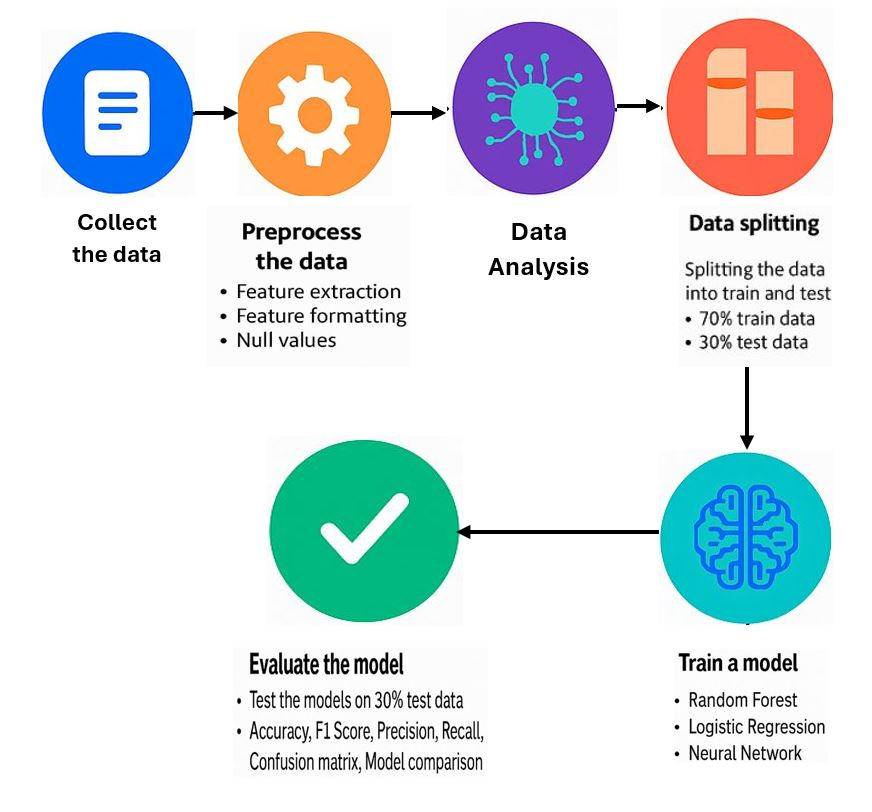
\includegraphics[height=7cm,width=8cm]{Flowchart.JPG}
\caption{Our Research Workflow} 
\label{fig:Our Research Workflow}
\end{figure}



\section{Data Analysis and Pre-Processing}

This research makes use of freely available dataset on Kaggle website~\cite{8} ~\cite{9}. Their testbed infrastructure has been split, as Fig.~\ref{fig:architecture} shows, into two entirely different networks: Attack-Network and Victim-Network. Here, the Victim-Network they included all common and required devices, including router, firewall, switch, along with the several versions of the common three operating systems namely Windows, Linux and Macintosh.

\begin{figure}[htbp]
\centerline{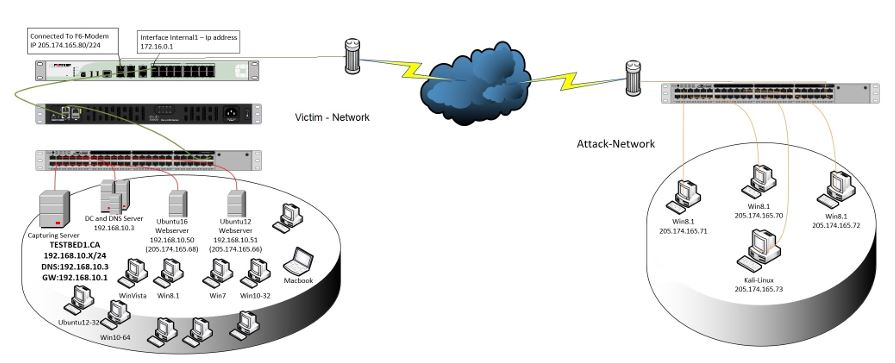
\includegraphics[height=4cm,width=8cm]{TestedArchitecture.JPG}}
\caption{Testbed Architecture: Victim and Attack Networks ~\cite{13}}
\label{fig:architecture}
\end{figure}

Table~\ref{tab:machine_setup} lists the servers, workstations, firewall, installed operating systems, related public and private IPs. Comprising one router, one switch, four PCs running Kali and Windows 8.1, the Attack-Network. Three servers, one firewall, two switches, ten PCs coupled by a domain controller (DC) and active directory make up the Victim-Network. One port in the Victim-Network's main switch has also been set as the mirror port and has entirely catches all send and receive traffic to the network.
\begin{table}[htbp]
\caption{Machine Setup of Victim and Attacker Networks ~\cite{13}}
\label{tab:machine_setup}
\centering
\resizebox{\linewidth}{90}{%
\begin{tabular}{|c|c|c|}
\hline
\textbf{Machine} & \textbf{OS} & \textbf{IPs} \\
\hline
\multirow{10}{*}{\textbf{Victim-Network}} 
  & \multicolumn{2}{1|}{\textbf{Servers}} \\
\cline{2-3}
  & Win Server 2016 (DC and DNS) & 192.168.10.3 \\
\cline{2-3}
  & Ubuntu 16 (Web Server) & 192.168.10.50 -- 205.174.165.68 \\
\cline{2-3}
  & Ubuntu 12 & 192.168.10.51 -- 205.174.165.66 \\
\cline{2-3}
  & \multicolumn{2}{1|}{\textbf{PCs}} \\
\cline{2-3}
  & Ubuntu 14.4 (32, 64) & 192.168.10.19 -- 192.168.10.17 \\
\cline{2-3}
  & Ubuntu 16.4 (32-64) & 192.168.10.16 \\
\cline{2-3}
  & Win 7Pro & 192.168.10.12 \\
\cline{2-3}
  & Win 8.1-64 & 192.168.10.9 \\
\cline{2-3}
  & Win Vista & 192.168.10.8 \\
\cline{2-3}
  & Win 10 (Pro 32-64) & 192.168.10.14 \\
\cline{2-3}
  & Mac & 192.168.10.25 \\
\hline
\multirow{1}{*}{\textbf{Firewall}} 
  & Fortinet & \\
\hline
\multirow{5}{*}{\textbf{Attackers}} 
  & \multicolumn{2}{1|}{\textbf{PCs}} \\
\cline{2-3}
  & Kali & 205.174.165.73 \\
\cline{2-3}
  & Win 8.1 & 205.174.165.70 \\
\cline{2-3}
  & Win 8.1 & 205.174.165.71 \\
\cline{2-3}
  & Win 8.1 & 205.174.165.71 \\
\hline
\end{tabular}
} % end resizebox
\end{table}



Over a five-day period, Monday through Friday, the experimental setup was carried out under which an extensive range of cyberattacks were systematically launched against the victim network. Monday was set aside as a control day, as Table~\ref{tab:attack_days} shows, and only normal, benign network traffic. Beginning Tuesday through Friday, a sequence of strikes was executed at several times of day to replicate real-world threat scenarios. Brute Force attacks on FTP and SSH protocols, Denial-of-Service (DoS) attacks, Heartbleed vulnerability exploits, varied Web-based attacks, SQL Injections, Infiltration techniques, Botnet activities including ARES, and large-scale Distributed Denial-of-Service (DDoS) attacks comprised these strikes. Every kind of attack was carried out in the morning and afternoon sessions of the corresponding days to vary the attack patterns and augment the dataset with different hostile traffic. This time-based attack structure allows a comprehensive evaluation of intrusion detection models in multiple types of threats and traffic patterns.~\cite{13}


\begin{table}[htbp]
\caption{Attack Types by Day}
\label{tab:attack_days}
\centering
\begin{tabular}{|c|p{5.8cm}|}
\hline
\textbf{Day} & \textbf{Labels} \\
\hline
Monday & Benign \\
\hline
Tuesday & BForce, SFTP and SSH \\
\hline
Wednesday & DoS and Heartbleed Attacks: slowloris, Slowhttptest, Hulk and GoldenEye \\
\hline
Thursday & Web and Infiltration Attacks: Web BForce, XSS and SQL Inject. Infiltration Dropbox Download and Cool disk \\
\hline
Friday & DDoS LOIT, Botnet ARES, PortScans (sS, sT, sF, sX, sN, sP, vS, vU, sO, sA, sW, sR, sL and B) \\
\hline
\end{tabular}
\end{table}

We used the network traffic data especially from Wednesday, which is available as a separate part on the Kaggle platform, for model development. This particular day the dataset was generated by running multiple types of Denial-of-Service (DoS) and Heartbleed attacks. These consisted in attacks from Slowloris, Slowhttptest, Hulk, and GoldenEye. Every one of these attack techniques has a unique label in the dataset, so allowing a fine-grained classification method. CICFlowMeter, a flow generator tool that pulls thorough statistical features from network packets, handled the raw network traffic. Along with a label field, the tool generated 80 features overall for every flow. Every flow record in the dataset consists in identifying metadata including source IP, source port, destination IP, destination port, and protocol applied. The dataset has 80 columns in all and 692{,}704 rows. Data exploration and selection criteria helped one to find, as Table~\ref{tab:important_features} shows, the most important characteristics. To improve the specificity of the classification task, we thus concentrated just on data samples labeled as DoS attacks, so excluding other attack types for the scope of this study.
\begin{table}[htbp]
\caption{Most Important Features for Each Attack Label ~\cite{13}}
\label{tab:important_features}
\centering
\renewcommand{\arraystretch}{1.5}  % Decrease row height
\resizebox{\linewidth}{!}{%
\begin{tabular}{|c|l|}
\hline
\textbf{Label} & \textbf{Feature} \\
\hline
Benign & B.Packet Len Min, Subflow F.Bytes, Total Len F.Packets, F.Packet Len Mean \\
\hline
DoS GoldenEye & B.Packet Len Std, Flow IAT Min, Fwd IAT Min, Flow IAT Mean \\
\hline
Heartbleed & B.Packet Len Std, Subflow F.Bytes, Flow Duration, Total Len F.Packets \\
\hline
DoS Hulk & B.Packet Len Std, B.Packet Len Std, Flow Duration \\
\hline
DoS Slowhttp & Flow IAT Std, Flow Duration, Active Min, Active Mean \\
\hline
DoS slowloris & F.IAT Min, F.IAT Mean, Init Win F.Bytes, Subflow F.Bytes \\
\hline
SSH-Patator & Total Len F.Packets, ACK Flag Count, Init Win F.Bytes \\
\hline
FTP-Patator & F.PSH Flags, SYN Flag Count, F.Packets/s \\
\hline
Web Attack & Init Win F.Bytes, Subflow F.Bytes, Total Len F.Packets \\
\hline
Infiltration & Subflow F.Bytes, Total Len F.Packets, Flow Duration, Active Mean \\
\hline
Bot & Subflow F.Bytes, Total Len F.Packets, F.Packet Len Mean, B.Packets/s \\
\hline
PortScan & Init Win F.Bytes, B.Packets/s, PSH Flag Count \\
\hline
DDoS & B.Packet Len Std, Avg Packet Size, Flow Duration, Flow IAT Std \\
\hline
\end{tabular}
}
\end{table}


The \texttt{df.replace()} feature was used to handle infinite and null values that might interfere with the learning process, so preparing the dataset for model training. This phase guarantees appropriate replacement or elimination of any instances of \texttt{inf}, \texttt{-inf}, or \texttt{NaN} in the dataset. Following missing values, the \texttt{Label} column received binary mapping in which all DDoS-related attacks received a value 1 and benign or normal traffic received a value 0. This improvement turns the multi-class problem into a binary classification challenge. To ensure the consistency and quality of the training data, all rows that shifted from the defined label mapping were removed from the dataset.

\begin{center}
\begin{scriptsize}
\begin{verbatim}
label_map = {
    'BENIGN': 0,
    'DoS Hulk': 1,
    'DoS GoldenEye': 1,
    'DoS slowloris': 1,
    'DoS Slowhttptest': 1,
    'Heartbleed': 1
}
df['Label'] = df['Label'].map(label_map)
df = df.dropna(subset=['Label'])
\end{verbatim}
\end{scriptsize}
\end{center}



For compatibility with machine learning algorithms, all feature columns were processed following label transformation. Models like Random Forest and Logistic Regression call for numerical input, thus all features had to be converted into numerical form. To reach this, during the conversion process non-numeric entries—such as strings or possibly corrupted data—were forced into \texttt{NaN} values. Some columns thus came totally composed of missing values. These columns were removed from the dataset later on without any useful information in order to maintain data quality to avoid errors during model training. This step ensured that only valid, numeric features were retained for the classification task.

\begin{scriptsize}
\begin{verbatim}
X = df.drop('Label', axis=1).apply(pd.to_numeric, 
errors='coerce')
y = df['Label'].astype(int)

# Remove columns with all NaN values
X = X.dropna(axis=1, how='all')
\end{verbatim}
\end{scriptsize}


Figures~\ref{fig:raw_data} and~\ref{fig:processed_data} illustrate the distribution of the raw dataset and the processed dataset, respectively. These visualizations provide a comparative view of the data before and after cleaning and preprocessing.

\begin{figure}[htbp]
\centerline{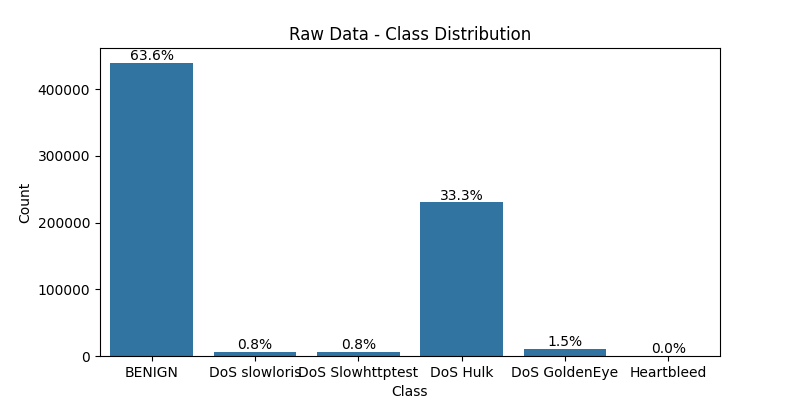
\includegraphics[width=0.52\textwidth]{Raw_Data_Distribution.png}}
\caption{Distribution of Raw Dataset}
\label{fig:raw_data}
\end{figure}

\begin{figure}[htbp]
\centerline{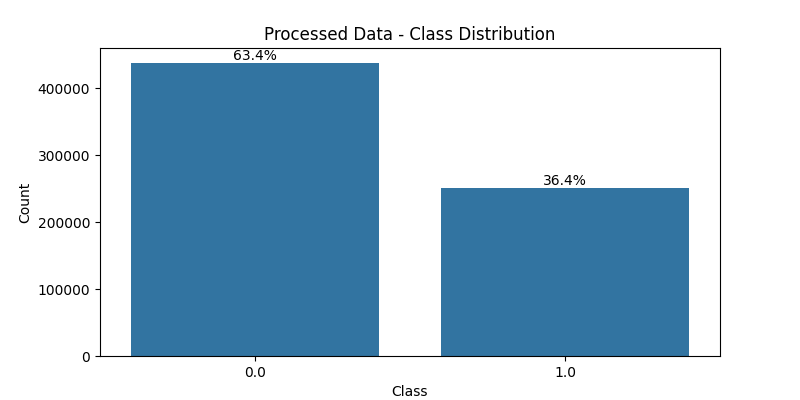
\includegraphics[width=0.52\textwidth]{Processed_Data_Distribution.png}}
\caption{Distribution of Processed Dataset}
\label{fig:processed_data}
\end{figure}

After the preprocessing process and cleaning, the dataset was split into training and testing subsets with the scikit-learn library's \texttt{train\_test\_split()} method. A stratified sampling technique was used to guarantee that the target labels—benign and DoS attack—remained consistent in both subsets. By applying a 70:30 ratio—that is, 30\% for testing and 70\% for training—the data was split. The random state was fixed to ensure reproducibility of the split.
\begin{center}
\begin{scriptsize}
\begin{verbatim}
from sklearn.model_selection import train_test_split

# Split the preprocessed data into training and testing sets
X_train, X_test, y_train, y_test = train_test_split(
    X, y,
    test_size=0.3,         # 30% for testing
    stratify=y,            # preserve label distribution
    random_state=42        # reproducibility
)
\end{verbatim}
\end{scriptsize}
\end{center}




\section{Structure of Model}

In a supervised learning system, classification algorithms form a major component of both training and testing stages. Classifiers use learned knowledge from labeled training data to project results on unprocessed test data. We present the classifiers used in this subsection to classify network traffic as either benign or suggestive of a DDoS attack. Designed to classify inputs into predefined groups depending on learnt patterns, a classifier is a machine learning model. In our situation, the classifier forecasts whether a given flow of network traffic is normal or related with a DoS attack. We used the Random Forest Classifier, Logistic Regression, and Multi-layer Perceptron (Neural Network) machine learning algorithms to achieve this.

\subsection*{1) Random Forest Classifier} Code in bellow displays Python implementation of the Random Forest Classifier applied to identify DoS-based DDoS attacks. Instantiated with \texttt{RandomForestClassifier()} with parameters including 100 estimators and a maximum depth of 15 to balance performance and overfitting, the classifier. The model was trained using the \texttt{fit()} method on the training data (\texttt{X\_train}, \texttt{y\_train}) and subsequently assessed by means of predictions on the test data (\texttt{X\_test}) employing the \texttt{predict()} method.

\begin{center}
\begin{scriptsize}
\begin{verbatim}
# Initialize and train Random Forest Classifier
rf_model = RandomForestClassifier(
    n_estimators=100,
    max_depth=15,
    n_jobs=-1,
    random_state=42,
    verbose=1
)
rf_model.fit(X_train, y_train)

# Evaluate Random Forest Classifier
rf_pred = rf_model.predict(X_test)
rf_metrics = {
    'Accuracy': accuracy_score(y_test, rf_pred),
    'F1 Score': f1_score(y_test, rf_pred),
    'Precision': precision_score(y_test, rf_pred),
    'Recall': recall_score(y_test, rf_pred)
}
\end{verbatim}
\end{scriptsize}
\end{center}


Using \texttt{accuracy\_score()}, the evaluation process computed the accuracy; it then created a confusion matrix using \texttt{confusion\_matrix()} and evaluated detailed performance metrics using \texttt{classification\_report()}, so offering precision, recall, F1-score, and support for every class. The results showed that the Random Forest model performed consistently well in classifying DDoS and benign traffic, demonstrating strong generalization capabilities and high classification accuracy.



\subsection*{2) Logistic Regression Classifier}

Bellow code of the application of the Logistic Regression classifier for binary network traffic. To ensure proper convergence during training, the model was trained using the \texttt{LogisticRegression()} function with a high iteration limit, \texttt{max\_iter=1000}. Predictions were generated on the test set using \texttt{predict()} following appropriate model fit to the training set. For overall accuracy, the evaluation phase used \texttt{accuracy\_score()}; for precision, recall, and F1-score analysis, \texttt{classification\_report()}. Additionally produced to show the classification result was a confusion matrix. Logistic regression performed well in linearly separable patterns throughout the dataset even if it is a simpler model than ensemble and neural network methods. It provided a strong basis with fast computation and interpretability that kept competitive accuracy in DDoS traffic detection.

\begin{center}
\begin{scriptsize}
\begin{verbatim}
# Initialize and train Logistic Regression Classifier
lr_model = LogisticRegression(
    max_iter=1000,
    random_state=42
)
lr_model.fit(X_train, y_train)

# Evaluate Logistic Regression Classifier
lr_pred = lr_model.predict(X_test)
lr_metrics = {
    'Accuracy': accuracy_score(y_test, lr_pred),
    'F1 Score': f1_score(y_test, lr_pred),
    'Precision': precision_score(y_test, lr_pred),
    'Recall': recall_score(y_test, lr_pred)
}
\end{verbatim}
\end{scriptsize}
\end{center}


\subsection*{3) Neural Network (MLP Classifier)}

The Multi-layer Perceptron (MLP) Classifier, a feedforward neural network applied for more complicated pattern recognition in the dataset, bellow code through training and evaluation. The model used early stopping to prevent overfitting and was built with \texttt{MLPClassifier()} with two hidden layers totaling 100 and 50 neurons. \texttt{fit()} was used in training on the training dataset; \texttt{predict()} was used on the test set. Standard metrics—accuracy, precision, recall, F1-score—as well as visualization of the confusion matrix—were used to evaluate the model. Deep structure allowed the MLP model to capture nonlinear relationships in the data and provided strong performance in recognizing complicated DDoS traffic patterns.

\begin{center}
\begin{scriptsize}
\begin{verbatim}
# Initialize and train Neural Network Classifier
nn_model = MLPClassifier(
    hidden_layer_sizes=(100, 50),
    max_iter=500,
    early_stopping=True,
    random_state=42,
    verbose=True
)
nn_model.fit(X_train, y_train)

# Evaluate Neural Network Classifier
nn_pred = nn_model.predict(X_test)
nn_metrics = {
    'Accuracy': accuracy_score(y_test, nn_pred),
    'F1 Score': f1_score(y_test, nn_pred),
    'Precision': precision_score(y_test, nn_pred),
    'Recall': recall_score(y_test, nn_pred)
}
\end{verbatim}
\end{scriptsize}
\end{center}



\section{Performance Measurement}

The performance of the suggested machine learning models in identifying DDoS attacks is measured in this study using several kinds of evaluation metrics. These consist of the area under the ROC curve (AUC), F1-score, recall, accuracy, and precision. When used to identify DDoS-related traffic, these metrics and the confusion matrix offer an in-depth understanding of each classifier's effectiveness and reliability. The evaluation output includes both the model’s overall accuracy and a detailed classification report that summarizes the model’s ability to distinguish between benign and malicious network flows ~\cite{10}.

\begin{itemize}
    \item \textbf{Accuracy (ACC)} represents the overall success rate of the classifier and is defined as:

    \[
    \text{Accuracy} = \frac{TP + TN}{TP + TN + FP + FN}
    \]

    where TP denotes true positives, true negatives of TN, false positives of FP and false negatives of FN. This metric reflects the proportion of total instances correctly classified by the model.

    \item \textbf{Precision (P)} measures the reliability of positive predictions and is calculated as:

    \[
    \text{Precision} = \frac{TP}{TP + FP}
    \]

    It indicates how many of the instances predicted as DDoS attacks are actually DDoS, offering insight into the classifier’s ability to avoid false alarms.
    

    \item \textbf{Recall (R)}, also known as sensitivity or true positive rate, is a measure of the classifier’s ability to detect all actual DDoS attacks:

    \[
    \text{Recall} = \frac{TP}{TP + FN}
    \]

    It quantifies the proportion of actual attack instances correctly identified, making it crucial for minimizing missed detections.
\begin{figure}[htbp]
\centerline{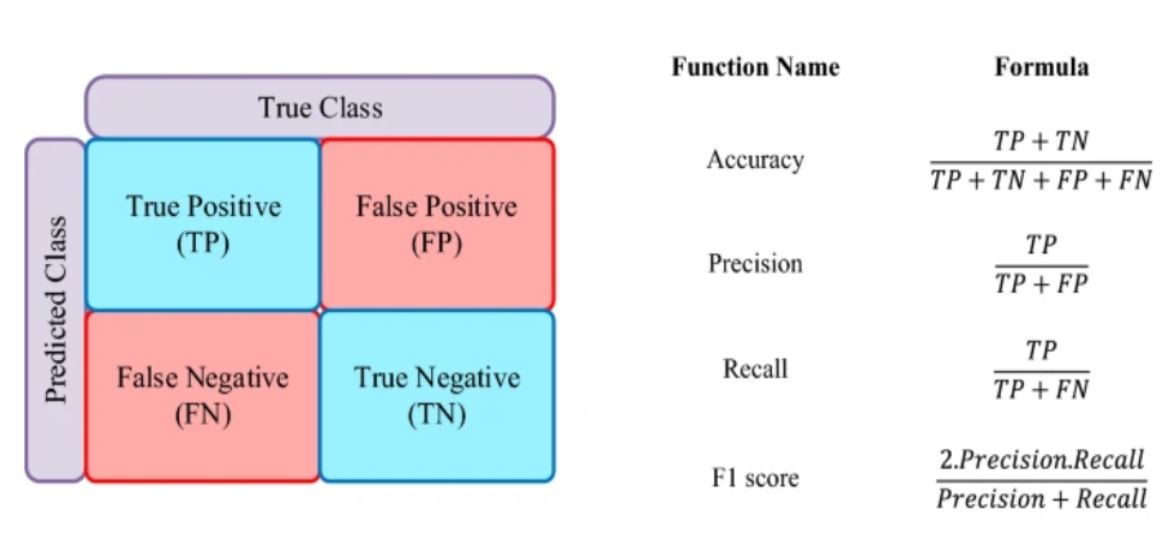
\includegraphics[width=0.45\textwidth]{ConfussionMatrix.JPG}}
\caption{Confusion matrix and performance metrics formula}
\label{fig:ConfusionFormula}
\end{figure}
    \item \textbf{F1 Score} is the harmonic mean of precision and recall:

    \[
    \text{F1 Score} = \frac{2 \cdot \text{Precision} \cdot \text{Recall}}{\text{Precision} + \text{Recall}}
    \]

    This metric provides a balanced view of the model’s performance, particularly in imbalanced datasets where relying on accuracy alone may be misleading.

\begin{center}
\begin{scriptsize}
\begin{verbatim}
def save_confusion_matrix(y_true, y_pred, model_name):
    """Save confusion matrix as image."""
    cm = confusion_matrix(y_true, y_pred)
    plt.figure(figsize=(8, 6))
    sns.heatmap(cm, annot=True, fmt='d', cmap='Blues',
                xticklabels=['Benign', 'DDoS'],
                yticklabels=['Benign', 'DDoS'])
    plt.title(f'{model_name} Confusion Matrix')
    plt.xlabel('Predicted')
    plt.ylabel('Actual')

    os.makedirs('results', exist_ok=True)
    plt.savefig(f'results/{model_name.replace
    (" ", "_")}_CM.png')
    plt.close()
\end{verbatim}
\end{scriptsize}
\end{center}


    \item \textbf{Area Under the ROC Curve (AUC)} is another vital evaluation metric used in this study. The trade-off between true positive rate (Recall) and false positive rate at various threshold settings is depicted by the Receiver Operating Characteristic (ROC) curve. The model's overall ability to differentiate between classes is determined by the AUC. A better-performing model can be determined by a higher AUC value, which indicates the classifier's increased ability to accurately differentiate between attack and normal traffic. To evaluate each model's performance and robustness visually, ROC curves were developed and compared.


\end{itemize}
    
\begin{center}
\begin{scriptsize}
\begin{verbatim}
def save_roc_curves(models, X_test, y_test):
    """Generate and save ROC curve comparison."""
    plt.figure(figsize=(10, 6))
    colors = cycle(['blue', 'green', 'red'])

    for (name, model), color in zip(models.items(), colors):
        try:
            proba = model.predict_proba(X_test)[:, 1]
            fpr, tpr, _ = roc_curve(y_test, proba)
            roc_auc = auc(fpr, tpr)
            plt.plot(fpr, tpr, color=color,
                     label=f'{name} (AUC = {roc_auc:.2f})')
        except AttributeError:
            print(f"{name} model does 
            not have predict_proba.")
            continue
\end{verbatim}
\end{scriptsize}
\end{center}


These metrics were used to evaluate the performance of Random Forest, Logistic Regression, and Neural Network classifiers. The confusion matrix for the Random Forest Classifier produced it possible to precisely calculate all performance metrics by clearly separating the counts of true positives and true negatives from false positives and false negatives. The model's robustness and generalization ability in detecting DDoS traffic was shown by its high accuracy and robust F1-score. Despite its simplicity, the Logistic Regression model demonstrated competitive performance and quick convergence, as evidenced by its confusion matrix, which showed efficient detection with fewer false positives. Because of its nonlinear structure, the Neural Network Classifier may be able to identify more complex patterns in the data. Its effectiveness during situations where precision and recall trade-offs are crucial can be seen by its performance, which was represented by its ROC curve and metrics, which indicated strong recall and F1-score.




\section{Experimentation Results}

A real-world dataset collected at CICIDS 2017 was used for training and evaluating the suggested machine learning models for DDoS attack detection. Data preprocessing included handling missing values, label encoding, and robust feature scaling using the \texttt{RobustScaler} to normalize the dataset and reduce the influence of outliers. To ensure a balanced class distribution during both training and evaluation phases, the dataset was then stratified using \texttt{train\_test\_split(X, y, test\_size=0.3, random\_state=42)} to create 70\% training and 30\% testing subsets.

\begin{table}[htbp]
\caption{Classification Results}
\label{tab:classification_results}
\centering
\begin{tabular}{|l|c|c|c|c|}
\hline
\textbf{Classifier} & \textbf{Accuracy} & \textbf{Precision} & \textbf{Recall} & \textbf{F1-Score} \\
\hline
Random Forest & 0.9995 & 0.9989 & 0.9997 & 0.9993 \\
Neural Network & 0.9882 & 0.9827 & 0.9849 & 0.9838 \\
Logistic Regression & 0.9177 & 0.9095 & 0.8595 & 0.8838 \\
\hline
\end{tabular}
\end{table}

Standard classification metrics, such as accuracy, precision, recall, and F1-score, were used to compare the performance of three machine learning classifiers: Random Forest, Logistic Regression, and Neural Network (MLPClassifier). These metrics, which originated from each classifier's confusion matrix, provided an in-depth evaluation of how effectively they detected DDoS traffic.

\begin{figure}[htbp]
\centerline{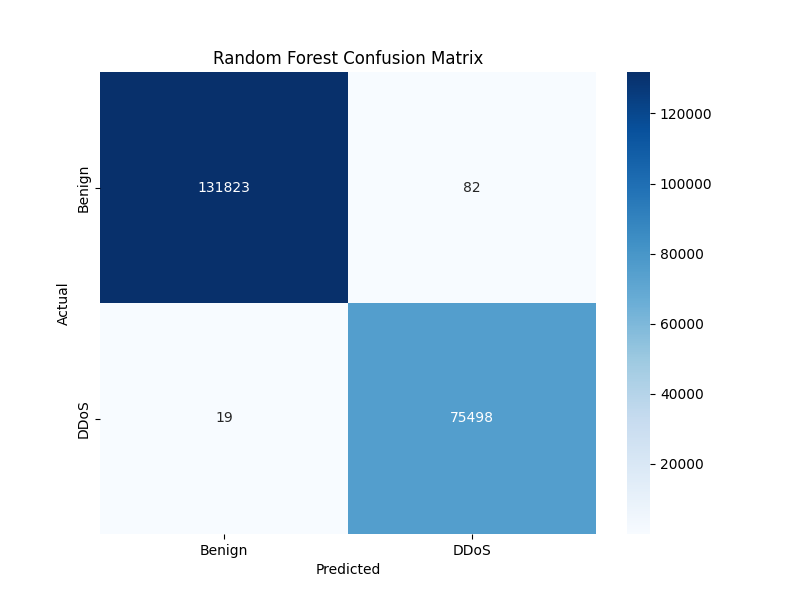
\includegraphics[width=0.45\textwidth]{Random_Forest_CM.png}}
\caption{Confusion Matrix for Random Forest Classifier}
\label{fig:rf_confusion}
\end{figure}

Table~\ref{tab:classification_results} presents the classification metrics for each model and summarizes the experiment results. With an accuracy of 99.95\%, precision of 99.89\%, recall of 99.97\%, and F1-score of 99.93\%, the Random Forest Classifier showed almost perfect accuracy and produced excellent outcomes. The Random Forest model's confusion matrix, as seen in Figure~\ref{fig:rf_confusion}, shows minimal misclassification, showing a high degree of reliability in distinguishing between malicious and benign traffic.

The Neural Network Classifier also delivered strong results with an accuracy of 98.82\%, precision of 98.27\%, recall of 98.49\%, and an F1-score of 98.38\%, as shown in Figure~\ref{fig:nn_confusion}. The confusion matrix highlights its effectiveness in capturing complex traffic patterns, although with slightly more misclassified instances compared to Random Forest.

On the other hand, the Logistic Regression Classifier achieved an accuracy of 91.77\%, precision of 90.95\%, recall of 85.95\%, and F1-score of 88.38\%, which, although lower than the other two models, still demonstrated acceptable performance, especially given its simplicity and computational efficiency. Figure~\ref{fig:lr_confusion} illustrates the corresponding confusion matrix for Logistic Regression.

\begin{figure}[htbp]
\centerline{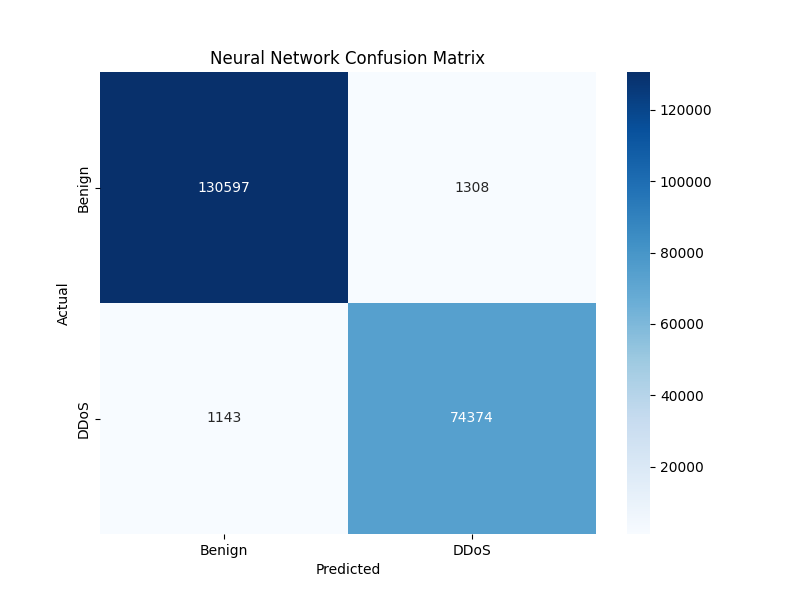
\includegraphics[width=0.45\textwidth]{Neural_Network_CM.png}}
\caption{Confusion Matrix for Neural Network Classifier}
\label{fig:nn_confusion}
\end{figure}

\begin{figure}[htbp]
\centerline{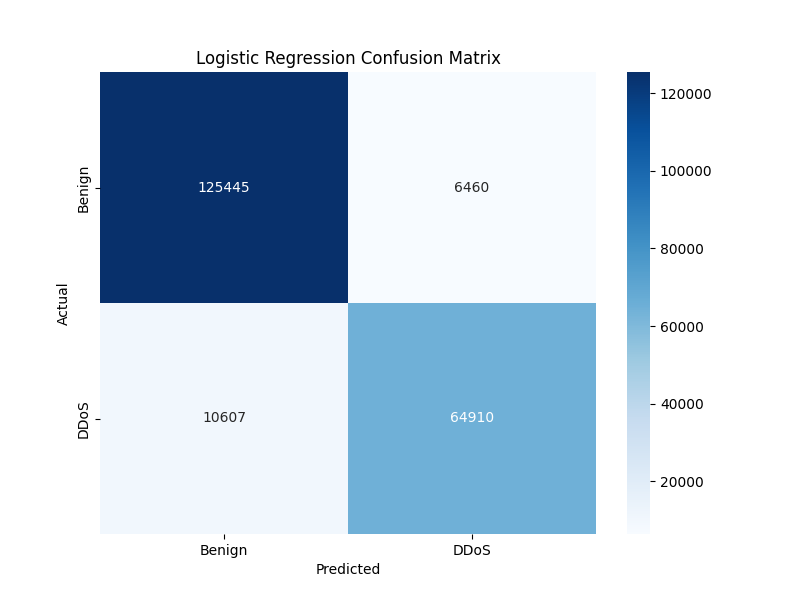
\includegraphics[width=0.45\textwidth]{Logistic_Regression_CM.png}}
\caption{Confusion Matrix for Logistic Regression Classifier}
\label{fig:lr_confusion}
\end{figure}

To further compare the models, the Receiver Operating Characteristic (ROC) curves were plotted for all three classifiers, as shown in Figure~\ref{fig:roc_curve}. The Area Under the Curve (AUC) values were 1.00 for Random Forest, 0.99 for Neural Network, and 0.92 for Logistic Regression. The ROC analysis confirms the superior classification ability of the Random Forest and Neural Network classifiers, especially in distinguishing true positives from false positives under various threshold settings.

\begin{figure}[htbp]
\centerline{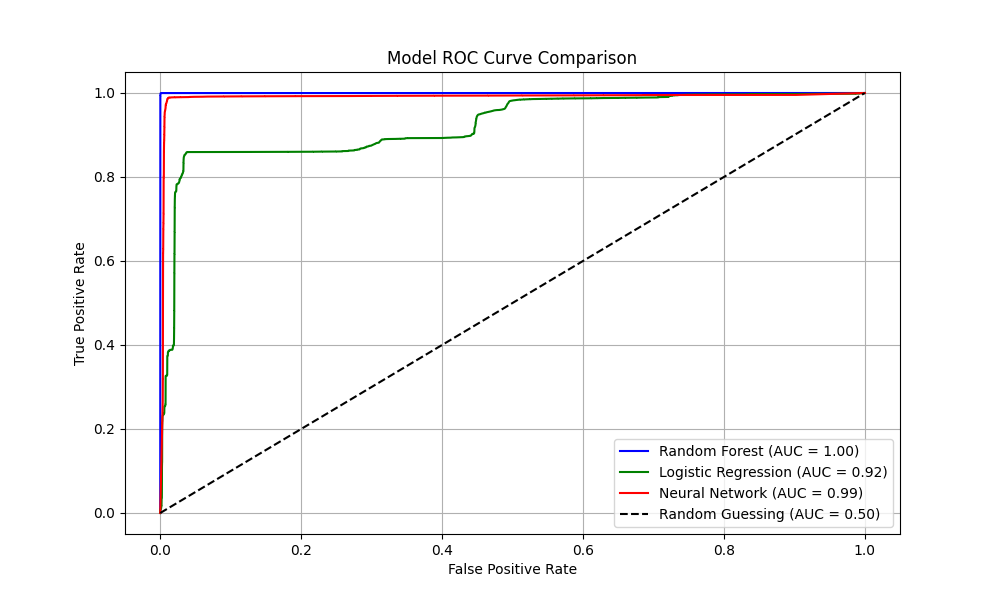
\includegraphics[width=0.45\textwidth]{ROC_Comparison.png}}
\caption{ROC Curve Comparison for Random Forest, Neural Network, and Logistic Regression Classifiers}
\label{fig:roc_curve}
\end{figure}






\section{Conclusion and Future Work}

In this study, we used network traffic data from the CICIDS 2017 dataset to show a machine learning-based method for identifying Distributed Denial-of-Service (DDoS) attacks. The accuracy, precision, recall, F1-score, and AUC of three classification models—Random Forest, Logistic Regression, and Neural Network (MLPClassifier)—were evaluated. With an accuracy of 99.95\% and almost perfect classification results, the Random Forest classifier outperformed the other models. It also scored highly on all evaluation metrics. While Logistic Regression, despite being simpler, maintained respectable performance with an accuracy of 91.77\%, the Neural Network classifier also showed strong predictive capabilities with an accuracy of 98.82\%. These results show how well Random Forest and Neural Network models differentiate between DDoS and benign traffic patterns, providing reliable responses for proactive cybersecurity defense.

For future work, this study can be extended by incorporating larger and more diverse network traffic datasets that include additional types of attacks and more realistic traffic behavior. Further improving detection performance may involve looking into additional machine learning methods like Support Vector Machines (SVM), Gradient Boosting, or advanced Deep Learning models like Convolutional or Recurrent Neural Networks. Additionally, applying feature selection or dimensionality reduction techniques could help identify the most influential traffic characteristics, improving both model interpretability and efficiency. Continuous monitoring and automated response would be made simpler by integrating the trained models into cloud-native platforms or real-time intrusion detection systems (IDS). Finally, testing the system with artificial traffic generators or in real-world network environments may help assess its scalability and resilience. 




\begin{thebibliography}{99}

\bibitem{1}
Cloudflare, ``DDoS Attack Trends and Reports,'' 2024. [Online]. Available: \url{https://blog.cloudflare.com/tag/ddos-reports/}


\bibitem{2}
R. R. Brooks, I. Ozcelik, L. Yu, J. Oakley, and N. Tusing, ``Distributed Denial of Service (DDoS): A History,'' \textit{IEEE Annals of the History of Computing}, 2021. DOI: \url{https://doi.org/10.1109/mahc.2021.3072582}.

\bibitem{3}
L. F. Eliyan and R. Di Pietro, ``DoS and DDoS attacks in Software Defined Networks: A survey of existing solutions and research challenges,'' \textit{Future Generation Computer Systems}, vol. 122, 2021. DOI: \url{https://doi.org/10.1016/j.future.2021.03.011}.

\bibitem{4}
M. Gniewkowski, ``An Overview of DoS and DDoS Attack Detection Techniques,'' in \textit{Theory and Applications of Dependable Computer Systems}, Springer, 2020, pp. 233–241. DOI: \url{https://doi.org/10.1007/978-3-030-48256-5_23}.

\bibitem{5}
B. Mahesh, ``Machine Learning Algorithms - A Review,'' \textit{ResearchGate}, 2019. [Online]. Available: \url{https://www.researchgate.net/publication/344717762_Machine_Learning_Algorithms_-A_Review}

\bibitem{6}
T. Thomas, A. P. Vijayaraghavan, and S. Emmanuel, ``Applications of Decision Trees,'' in \textit{Machine Learning Approaches in Cyber Security Analytics}, Springer, 2019, pp. 157–184. DOI: \url{https://doi.org/10.1007/978-981-15-1706-8_9}.

\bibitem{7}
R. Praba, G. Darshan, T. Roshanraj, and B. Surya, ``Study On Machine Learning Algorithms,'' \textit{International Journal of Scientific Research in Computer Science, Engineering and Information Technology}, vol. 7, no. 3, pp. 67–72, 2021. DOI: \url{10.32628/CSEIT2173105}.

\bibitem{8}
C. H. N. (ChethuHN), ``Network Intrusion Dataset,'' \textit{Kaggle}, 2017. [Online]. Available: \url{https://www.kaggle.com/datasets/chethuhn/network-intrusion-dataset}

\bibitem{9}
University of New Brunswick, ``CICIDS 2017 Dataset,'' Canadian Institute for Cybersecurity, 2017. [Online]. Available: \url{https://www.unb.ca/cic/datasets/ids-2017.html}

\bibitem{10}
Z. Karimi, ``Confusion Matrix,'' 2021. [Online]. Available: \textit{The confusion matrix is a tool for predictive analysis in machine learning. In order to check the performance of a classification based machine learning model, the confusion matrix is deployed.}

\bibitem{11}
S. Singh, M. Gupta and D. K. Sharma, ``DDOS Attack Detection with Machine Learning: A Systematic Mapping of Literature,'' in \textit{2023 5th International Conference on Smart Systems and Inventive Technology (ICSSIT)}, Tirunelveli, India, 2023, pp. 939--945, doi: \url{10.1109/ICSSIT55814.2023.10060897}.

\bibitem{12}
M. Merkebaiuly, ``Overview of Distributed Denial of Service (DDoS) attack types and mitigation methods,'' \textit{InterConf}, pp. 494--508, 2024. doi: \url{10.51582/interconf.19-20.03.2024.048}.

\bibitem{13}
I. Sharafaldin, A. H. Lashkari, and A. A. Ghorbani, ``Toward Generating a New Intrusion Detection Dataset and Intrusion Traffic Characterization,'' in \textit{Proceedings of the 4th International Conference on Information Systems Security and Privacy (ICISSP)}, 2018, pp. 108--116.

\bibitem{14}
LoginRadius, ``What is a DDoS Attack and How to Mitigate it,'' [Online]. Available: \url{https://www.loginradius.com/blog/engineering/how-to-mitigate-ddosattack/}. [Accessed: Apr. 17, 2025].





\bibitem{15}
F5, Inc., ``What is a Web Application Firewall (WAF)?,'' [Online]. Available: \url{https://www.f5.com/glossary/web-application-firewall-waf}. [Accessed: Apr. 17, 2025].
\bibitem{16}
Radware, ``What is Bot Management and How Does it Work?,'' [Online]. Available: \url{https://www.radware.com/cyberpedia/bot-management/botmanagement/}. [Accessed: Apr. 17, 2025].




\end{thebibliography}




\end{document}
